\documentclass{report}
%\usepackage{fullpage}

\usepackage[top=1in, bottom=1in, left=1.25in, right=.75in]{geometry}

    \usepackage{fancyhdr}
    \pagestyle{fancy}
    \lhead{PSD 2.0}
    \chead{}
    \rhead{\fancyplain{}{\textit{\leftmark}}}
    
%\renewcommand{\familydefault}{\sfdefault}
%\usepackage[scaled=1]{helvet}
%\usepackage[helvet]{sfmath}
%\everymath={\sf}

\usepackage{parskip}
\usepackage[colorinlistoftodos]{todonotes}
\usepackage[colorlinks=true, allcolors=blue]{hyperref}

\usepackage{amsmath}
\usepackage{amsfonts}
\usepackage{amssymb}
\usepackage{bbm}
\usepackage{bm}
\usepackage{cleveref}
\usepackage{listings}
\usepackage{graphbox,graphicx}
\usepackage{siunitx}
\usepackage{subcaption}


\usepackage{xcolor}
\definecolor{halfgray}{gray}{0.55}
\definecolor{ipython_frame}{RGB}{207, 207, 207}

\usepackage{color}
\definecolor{eclipseBlue}{RGB}{42,0.0,255}
\definecolor{eclipseGreen}{RGB}{63,127,95}
\definecolor{eclipsePurple}{RGB}{127,0,85}



\lstdefinelanguage{iPython}{
    commentstyle=\color{cyan}\ttfamily,
    stringstyle=\color{red}\ttfamily,
    keepspaces=true,
    showspaces=false,
    showstringspaces=false,
    %
    rulecolor=\color{ipython_frame},
    frame=single,
    frameround={t}{t}{t}{t},
    framexleftmargin=6mm,
    numbers=left,
    numberstyle=\tiny\color{halfgray},
    %
    basicstyle=\scriptsize\ttfamily,
    keywordstyle=\color{green}\ttfamily,
}

\lstdefinelanguage{PSD}
{
  % list of keywords
  morekeywords={
    import,
    if,
    while,
    for,
    np
  },
  sensitive=false, % keywords are not case-sensitive
  morecomment=[l]{//}, % l is for line comment
  morecomment=[s]{/*}{*/}, % s is for start and end delimiter
  morestring=[b]" % defines that strings are enclosed in double quotes
}

\lstdefinestyle{Linux}
{
 backgroundcolor=\color{white},
 basicstyle=\scriptsize\color{black}\ttfamily,
    frame=trbl, % draw a frame at the top, right, left and bottom of the listing
  frameround=tttt, % make the frame round at all four corners
  framesep=4pt, % quarter circle size of the round corners
}

%%%%%%%%%%%%%%%%%%%%%%%%%%%%%%%%%%  NEW COMMANDS %%%%%%%%%%%%%%%%%%%%%%%%%%%%%%%%%%
\newcommand{\bA}{\textbf{A}}
\newcommand{\bM}{\textbf{M}} 
\newcommand{\bx}{\textbf{x}} 
\newcommand{\bb}{\textbf{b}} 
\newcommand{\br}{\textbf{r}}
\newcommand{\bu}{\textbf{u}}
\newcommand{\bv}{\textbf{v}}
\newcommand{\bt}{\boldsymbol t}
\newcommand{\bl}{\boldsymbol f}
\newcommand{\bnv}{N_{\text{v}}}
\newcommand{\bnd}{N_{\text{DOF}}}
\newcommand{\bnz}{N_{\text{nz}}}
\newcommand{\bgc}{G_{\text{c}}}
\newcommand{\buh}{\boldsymbol u^h}
\newcommand{\bvh}{\boldsymbol v^h}
\newcommand{\bwh}{\boldsymbol w^h}
\newcommand{\bqh}{\boldsymbol q^h}
\newcommand{\bz}{\textbf{z}}
\newcommand{\bp}{\textbf{p}}
\newcommand{\np}{N_\text{p}}
\newcommand{\wu}{\widehat{u}}
\newcommand{\wbu}{\widehat{\textbf{u}}}
\newcommand{\we}{\widehat{\varepsilon}}
\newcommand{\ws}{\widehat{\sigma}}
\newcommand{\wf}{\widehat{f}}
\newcommand{\bff}{\textbf{f}}
\newcommand{\fih}{ d^h}
\newcommand{\ttah}{ \theta^h}
\newcommand{\sig}{\boldsymbol{\sigma}}
\newcommand{\eps}{\boldsymbol{\varepsilon}} 
\newcommand{\dv}{\mathrm{d}\text{v}}
\newcommand{\ds}{\mathrm{d}\text{s}}
%%%%%%%%%%%%%%%%%%%%%%%%%%%%%%%%%%%%%%%%%%%%%%%%%%%%%%%%%%%%%%%%%%%%%%%%%%%%%%%%%%%


\title{PSD}
\author{Mohd Afeef Badri}
\setcounter{tocdepth}{2}



\begin{document}
\maketitle

\pagebreak
\tableofcontents
\pagebreak
\chapter{Introduction} 

\section{Introduction} 
PSD is a finite elements-based solid mechanics solver with capabilities of performing High Performance Computing (HPC) simulations with billions of unknowns. The kernel of PSD is wrapped around FreeFEM for finite element discretization, and PETSc for linear algebra/Preconditioning. PSD solver contains straightforward supports for static or dynamic simulations with linear  and nonlinear solid mechanics problems. Besides these hybrid-phase field fracture mechanics models have also been incorporated within PSD. For dynamics the generalized-$\alpha$ model  for time discretization is used, this models enable straightforward use of Newmark-$\beta$, central difference, or HHT as time discretization. PSD uses sate-of-the art domain-decomposition paradigm via vectorial finite elements for parallel computing and all solvers are  proven to scale quasi-optimally. PSD has proven scalabilty uptill 13,000 cores with largest problem solved containing over 5 Billion unknowns.

\section{History}
Development of PSD started in Feburary 2019 at CEA.  

\chapter{Installation}


PSD is built to work with Linux and Windows platforms. 

\section{Dependencies}

To install and work with PSD first check that you have installed all the dependencies. PSD depends on the following:   

\begin{itemize}
\item  {\ttfamily C++}    (version 4.8 or greater)
\item  {\ttfamily automake}
\item  {\ttfamily FreeFEM}
\item  {\ttfamily PETSc}      (optional)
\item  {\ttfamily Gmsh}
\item  {\ttfamily gnuplot}	(optional)
\item  {\ttfamily git}   
\end{itemize}


\section{PSD installation steps \label{sec:psd-install}}
Now that I have all the dependencies what next ?  

\begin{itemize}
\item  Go ahead and grab the latest copy of PSD. The code is hosted on CEA's internal git repository.

\begin{lstlisting}[style=Linux]
git clone https://codev-tuleap.intra.cea.fr/plugins/git/hpcseism/freefem.git  PSD-Sources
\end{lstlisting}

\item  Now goto the {\ttfamily PSD-Sources} folder and autoconf PSD within the  cloned folder

\begin{lstlisting}[style=Linux]
autoreconf -i
\end{lstlisting}

\item Configure  PSD within the  cloned folder
\begin{lstlisting}[style=Linux]
./configure
\end{lstlisting}
Note:   {\ttfamily ./configure will} install PSD in {\ttfamily  \$HOME/PSD } to change this directory use {\ttfamily  --prefix=Your/Own/Path } with {\ttfamily ./configure}. 


\item Make PSD directives
\begin{lstlisting}[style=Linux]
make FFINSTALLDIR=/usr/local/bin/ GMSH=/usr/bin/gmsh
\end{lstlisting}
Note: variable {\ttfamily FFINSTALLDIR} can be changed to the {\ttfamily FreeFEM} local path if installed locally. Similarly variable {\ttfamily  GMSH } can be changed for {\ttfamily  Gmsh}.
Note: Please use the new version of {\ttfamily Gmsh} (greater than version 4.3.0) from their official website.

\item Install PSD
\begin{lstlisting}[style=Linux]
make install
\end{lstlisting}


\item Check if installation is correct 
\begin{lstlisting}[style=Linux]
make check
\end{lstlisting}

Now you should have the solver at {\ttfamily \$HOME/PSD}. To use the solver please go to {\ttfamily \$HOME/PSD}.

\end{itemize}

\section{Update PSD to the latest version}

If you are a PSD user and would like to update your old PSD source to a new one. Go to your {\ttfamily PSD-Sources} folder and

\begin{lstlisting}[style=Linux]
git pull origin master
\end{lstlisting}

After this step simply

\begin{lstlisting}[style=Linux]
./reconfigure;  make;  make install;  make check
\end{lstlisting}

\section{Using PSD for brittle fracture}

If you plan to use PSD for brittle fracture simulations, you must tweak your FreeFEM installation.

\section{PSD installation for supercomputer}

To install a copy of PSD that will be used on a supercomputer/cluster. During the  {\ttfamily make} command of PSD from \cref{sec:psd-install} instead do 

\begin{lstlisting}[style=Linux]
make supercomp
\end{lstlisting}

Note that the copy of PSD installed is not complete. You will have to manually build the static libraries on the supercomputer. Once your PSD copy is on supercomputer, go to  {\ttfamily PSD/plugin} folder, and 
\begin{lstlisting}[style=Linux]
make
\end{lstlisting}





\chapter{Tutorials}

\textbf{Preliminaries}\\
Before diving into the tutorials, here are some preliminaries that will help you guide easily through them.

\begin{itemize}
    \item A PSD simulation is performed in three steps: preprocessing, solving, and postprocessing. 
    \item Domain: denoted by $\Omega$ is a a $n$-dimensional solid body such that $\Omega \subset \mathbbm{R}^n$ with $n=2$   for 2D problems or  $n=3$ for 3D problems.
    \item Finite element mesh: denoted by $\Omega^h$ with mesh size $h$. Mesh can be triangular in 2D and tetrahedral in 3D.
    \item MPI processes for simulation: denoted by $\np$ these are the total MPI ranks that will work parallely to solve the problem.
    \item Partitioned mesh: denoted by $\{ \Omega ^h_i \}_{i=1}^{\np}$ these are set of subdomains which are heald by each MPI rank during a parallel simulation.
\end{itemize}

\section{Linear Elasticity}
This is the basic model for solving simple solid mechanics. PSD allows for solving Linear Elasticity both in sequential and in parallel. We shall discuss how to do so in details within this section.


PSD is a FEM based solver, to solve a given physics it heavily relies on the variational formulations of the underlying physics. Let us begin with writing the variational formulation of system of  Elasticity in which the primary unknown is the displacements vector $\bu\{u_i\}^n_{i=1}$. In the Lagrangian FE framework for searching the unknown nodal displacements vector $\bu^h=\{u^h_i\}^n_{i=1}$ the variational formulation of system of  Elasticity reads,
%
%
\begin{equation}\label{Eq:VarfU}
\int_{\Omega^h_i}\sig(\buh) : \eps(\bvh) = \int_{\partial\Omega^h_{i,\text{N}}} \mathbf{f}\cdot\bvh \, \quad\forall\,\bvh\in\mathbb{V}^h,\buh\in\mathbb{V}^h,
\end{equation}
%
here, the nodal displacements vector $\buh$ is in fact the FE trial function and $\bvh=\{v^h_i\}^n_{i=1}$ is the FE test function.

\begin{equation}\label{Eq:LinearElasticity}
\int_{\Omega^h_i}\lambda\nabla\cdot\buh\nabla\cdot\bvh + \int_{\Omega^h_i}2\mu\boldsymbol\varepsilon(\buh):\boldsymbol\varepsilon(\bvh)-\int_{\Omega^h_i}\mathbf{f}\cdot\bvh=0, \quad\forall\bvh\in[H^1_0(\Omega^h_i)]^n 
\end{equation}

In these formulations $\lambda$ and $\mu$ are the Lame's parameters, $\mathbf{f}$ is the body force vector.  

\subsection{PSD simulation of 2D bar problem bending under own body weight \label{sec:2d-bar-load}}

To showcase the usage of Linear elasticity, we shall discuss here an example of a 2D bar, which bends under its own load. The bar ---$5\times1$~\si{\square\meter} in area-- is made up of material with $\rho=8\text E3$, $E=200\text E9$, and $\nu=0.3$.

\begin{figure}[htbp]
    \centering
    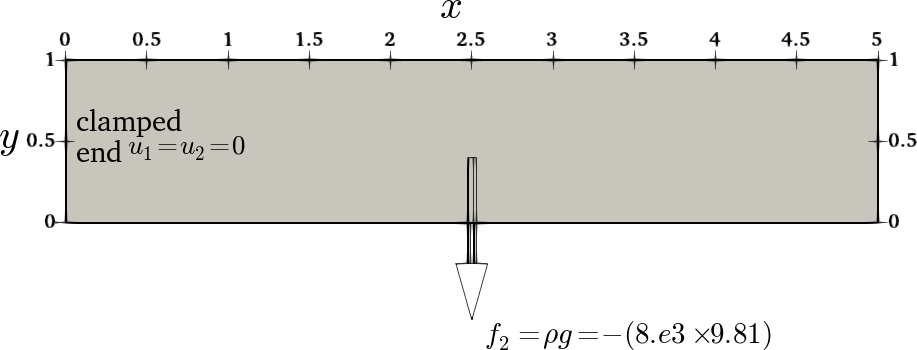
\includegraphics[align=t,width=.44\textwidth]{2d-bar.png}\hspace{.1\textwidth}
    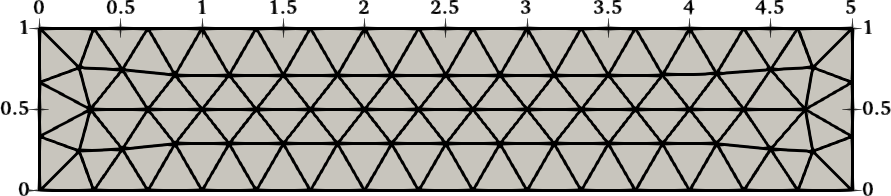
\includegraphics[align=t,width=.44\textwidth]{2d-bar-mesh.png}
    \caption{2D bar clamped at left end and bending under own load. Geometry (left) and mesh (right).}
    \label{fig:my_label}
\end{figure} 

\textbf{Step 1: Preprocessing}

First step in a PSD simulation is ``PSD setup", at this step you tell PSD what kind of physics, boundary conditions, approximations, mesh, etc are you expecting to solve.
For ``PSD setup" go to the {\ttfamily PSD/Solver} folder, launch the terminal there and run the following command.
\begin{lstlisting}[style=Linux]
PSD_PreProcess -dimension 2 -bodyforce  -dirichletconditions 1 -plot
\end{lstlisting}
%
After the ``PSD setup" runs successfully you should see many {\ttfamily .edp} files in your {\ttfamily PSD/Solver} folder. \textit{What do the arguments mean ?} {\ttfamily SolverGenerator.edp} is the file that is responsible for creating additional files in your {\ttfamily PSD/Solver} folder; {\ttfamily -dimension 2} means it is a 2D simulation, {\ttfamily -bodyforce} with body force; {\ttfamily -dirichletconditions 1} says we have one Dirichlet border; and {\ttfamily -plot} means we would like to have ParaView post processing files. The input properties ``$E,\nu, \mathbf{f}$" can be changed in {\ttfamily ControlParameters.edp} by changing {\ttfamily E, nu, f$_2$}. These are changed to {\ttfamily E  = 200.e9}, {\ttfamily nu = 0.3;}, {\ttfamily f$_2$=8.e3*(-9.81);}. Note, {\ttfamily f$_2$} is the second component of $\mathbf{f}$. Dirichlet boundary conditions are also provided in {\ttfamily ControlParameters.edp}. To provide Dirichlet label (clamped end), the vector {\ttfamily int[int] Dlabel = [2];} should be used, here we assume that the label number of the left end is 2. For this clamped end $u_1=u_2=0$, this is provided by {\ttfamily real[int]   Dvalue = [0.,0.];}.

\textbf{Step 2: Solving}

As PSD is a parallel solver, let us use  4 cores to solve the 2D bar case. To do so enter the following command:

\begin{lstlisting}[style=Linux]
ff-mpirun -np 4 Main.edp
\end{lstlisting}

Here {\ttfamily -np 4} denote the argument used to enter the number of cores. Note that if your problem is large use more cores. PSD has been tested upto 13,000 cores, surely you will now need that many for the 2D bar problem. 

\textbf{Step 3: Postprocessing}

PSD allows postprocessing of results in ParaView. After the step 2 mentioned above finishes. Launch ParaView and have a look at the  {\ttfamily .pvd} file in the  {\ttfamily PSD/Solver/VTUs\_DATE\_TIME} folder. 

\begin{figure}[htbp]
    \centering
    \begin{minipage}[t][2cm][t]{0.4\textwidth}
    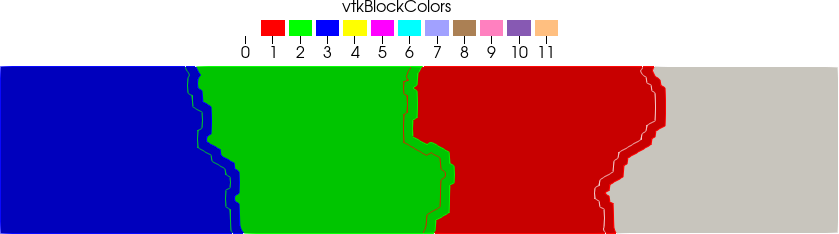
\includegraphics[align=t,width=1\textwidth]{2d-bar-partioned.png}
    \end{minipage}\hspace{.1\textwidth}
    \begin{minipage}[t][2cm][t]{0.4\textwidth}
    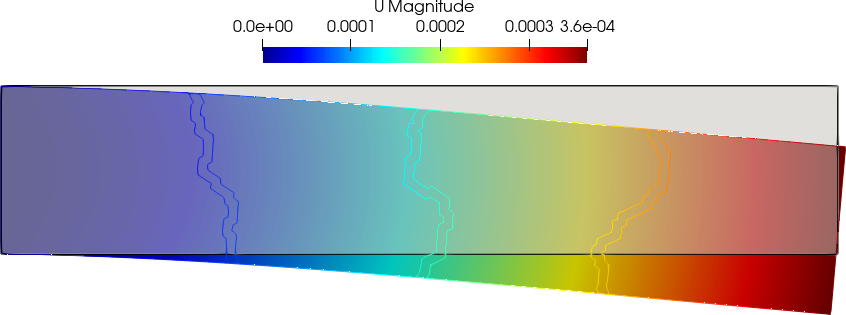
\includegraphics[align=t,width=1\textwidth]{2d-bar-results.png}
    \end{minipage}
    \caption{2D clamped bar results. Partitioned mesh (left) and 1000X warped displacement field (right).}
    \label{fig:my_label}
\end{figure}


\subsection{PSD simulation of 2D bar problem clamped at both ends \label{sec:2D-bar-clamped1}}

For this test the properties of the material are the same as used in \cref{sec:2d-bar-load}. 

\textbf{Step 1: Preprocessing}

For ``PSD setup" go to the {\ttfamily PSD/Solver} folder, launch the terminal there and run the following command.
\begin{lstlisting}[style=Linux]
PSD_PreProcess -dimension 2 -plot -dirichletconditions 2 -bodyforce
\end{lstlisting}
%
Since basic nature of both the problems is same this is the exact same command used in preprocessing of \cref{sec:2d-bar-load}. The only difference of this problem compared to the one from \cref{sec:2d-bar-load} is that an additional Dirichlet condition needs to be supplied, notified to PSD by {\ttfamily -dirichletconditions 2}. To provide Dirichlet label of the two clamped end in {\ttfamily ControlParameters.edp} the vector {\ttfamily int[int] Dlabel = [2,4];} should be used, here we assume that the label number of the left end is 2 and right end is 4. For these clamped end $u_1=u_2=0$, this is provided by {\ttfamily real[int]   Dvalue = [0.,0.,0.,0.];}. In the  {\ttfamily real[int]   Dvalue = [0.,0.,0.,0.];} the fist two digits correspond to $u_1,u_2$ of label 2 and the last two digits correspond to $u_1,u_2$ of label 4.



\textbf{Step 2: Solving}

Let us now use  3 cores to solve this problem. To do so enter the following command:

\begin{lstlisting}[style=Linux]
ff-mpirun -np 3 Main.edp
\end{lstlisting}
%
Notice, that this is the exact same command used in solving of \cref{sec:2d-bar-load}, with only difference that we now use {\ttfamily -np 3} vs.~{\ttfamily -np 4}.


\textbf{Step 3: Postprocessing}

Launch ParaView and have a look at the  {\ttfamily .pvd} file in the  {\ttfamily PSD/Solver/VTUs\_DATE\_TIME} folder. 

\begin{figure}[htbp]
    \centering
    \begin{minipage}[t][2cm][t]{0.4\textwidth}
    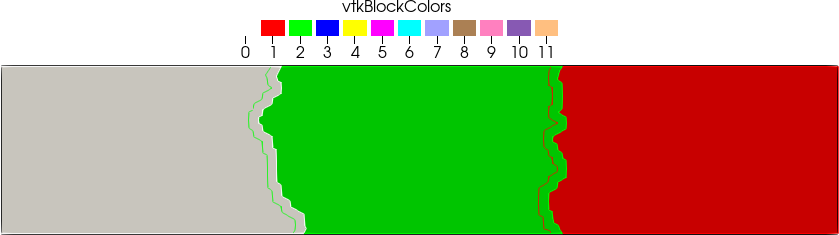
\includegraphics[align=t,width=1\textwidth]{2d-bar-partitioned3.png}
    \end{minipage}\hspace{.1\textwidth}
    \begin{minipage}[t][2cm][t]{0.4\textwidth}
    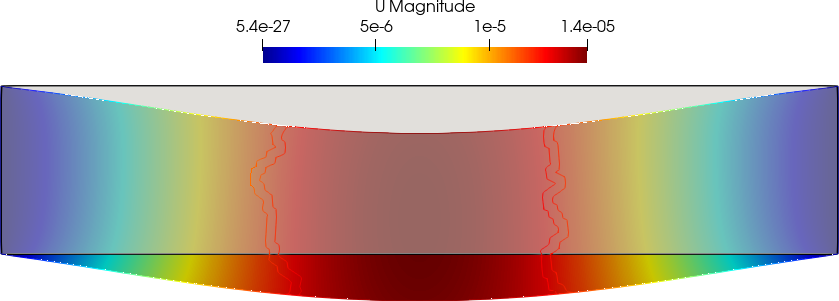
\includegraphics[align=t,width=1\textwidth]{2d-bar-clamped-ends.png}
    \end{minipage}
    \caption{2D clamped bar results. Partitioned mesh (left) and 20000X warped displacement field (right).}
    \label{fig:3part}
\end{figure}

In~\cref{fig:3part} there are only three subdomais in the partitioned mesh since only three cores were used.

\subsubsection{Redoing the test on Jupiter and moon}

Imagine, you wish to know how the test would compare if performed on Moon and Jupiter. The only thing that will change now is the gravitational pull, for Moon $g=1.32$ and for Jupiter $g=24.79$. To perform the moon test simply change  {\ttfamily f$_2$=8.e3*(-1.32);} in {\ttfamily ControlParameters.edp} and redo step 2 and step 3. Similarly for the Jupiter test {\ttfamily f$_2$=8.e3*(-24.79);} in {\ttfamily ControlParameters.edp} and redo step 2 and step 3.

\begin{figure}[htbp]
    \centering
    \begin{minipage}[t][2.5cm][t]{0.4\textwidth}
    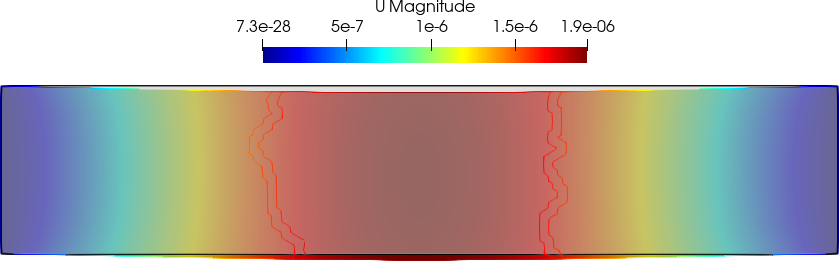
\includegraphics[align=t,width=1\textwidth]{2d-bar-moon.png}
    \end{minipage}\hspace{.1\textwidth}
    \begin{minipage}[t][2.5cm][t]{0.4\textwidth}
    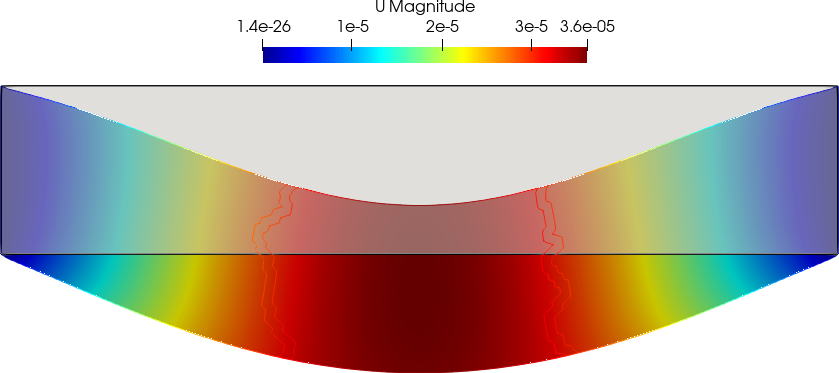
\includegraphics[align=t,width=1\textwidth]{2d-bar-Jupiter.png}
    \end{minipage}
    \caption{2D clamped bar 20000X warped displacement fields. On moon (left) and  on Jupiter (right).}
    \label{fig:moon-jupiter}
\end{figure}

\subsection{PSD simulation of 2D bar problem clamped at one end wile being pulled at the other end (Dirichlet-Dirichlet case)\label{sec:2d-bar-clamped2}}

In this section we showcase the 2D bar problem simulation with one end clamped wile being pulled at the other end. Body force is neglected and the non clamped ends pull is approximated with Dirichlet displacement $u_1=1$. If this simulation is compared to the previous one from \cref{sec:2d-bar-load}, the only difference now is that no body force is applied and an additional Dirichlet condition is applied at the free end of the bar. Here is how PSD simulation of this case can be performed.

\textbf{Step 1: Preprocessing}

For ``PSD setup" go to the {\ttfamily PSD/Solver} folder, launch the terminal there and run the following command.
\begin{lstlisting}[style=Linux]
PSD_PreProcess -dimension 2 -dirichletconditions 2 -plot
\end{lstlisting}
%
In comparison to preprocessing from \cref{sec:2d-bar-load,sec:2D-bar-clamped1}, notice that {\ttfamily -bodyforce} is missing. This is due to the fact that for this problem we assume zero body force. Just like in~\cref{sec:2D-bar-clamped1} {\ttfamily -dirichletconditions 2}, which notifies to PSD that there are two Dirichlet borders ---the clamped and the pulled ends of the bar--- in this simulation. To add the values and label numbers of the Dirichlet borders edit the  {\ttfamily ControlParameters.edp},  the vector {\ttfamily int[int] Dlabel = [2,4];} should be used, here we assume that the label number of the left end is 2 and right end is 4. For the left end $u_1=0,u_2=0$ and for the right end $u_1=1,u_2=0$, this is provided by {\ttfamily real[int]   Dvalue = [0.,0.,1.,0.];}. In the  {\ttfamily real[int]   Dvalue = [0.,0.,0.,0.];} the fist two digits correspond to $u_1,u_2$ of label 2 and the last two digits correspond to $u_1,u_2$ of label 4. Note that here at border 4 we have explicitly set $u_2=0$ this means the bar is not allowed to shrink in $y$ direction (compress), however you might wish to allow the bar to compress. Such a simulation requires a little bit of more editing in preprocessing step, we shall deal with this in the later tutorials, for now we focus on the current case. So now PSD should be ready to solve. 

\textbf{Step 2: Solving}

Let us now use 2 cores to solve this problem. To do so enter the following command:

\begin{lstlisting}[style=Linux]
ff-mpirun -np 2 Main.edp
\end{lstlisting}
%
Notice, that this is the exact same command used in solving of \cref{sec:2d-bar-load,sec:2D-bar-clamped1}, with only difference that we now use {\ttfamily -np 2} vs.~{\ttfamily -np 4} in \cref{sec:2d-bar-load} and ~{\ttfamily -np 3} in \cref{sec:2D-bar-clamped1}.


\textbf{Step 3: Postprocessing}

Launch ParaView and have a look at the  {\ttfamily .pvd} file in the  {\ttfamily PSD/Solver/VTUs\_DATE\_TIME} folder. 

\begin{figure}[htbp]
    \centering
    \begin{minipage}[t][2cm][t]{0.39\textwidth}
    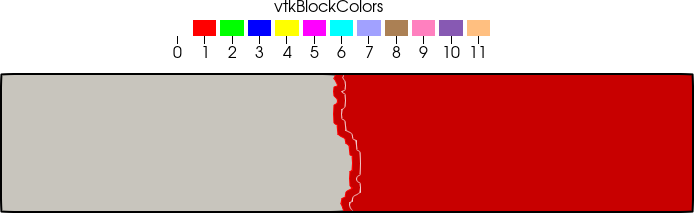
\includegraphics[align=t,width=1\textwidth]{2d-bar-clamped-pulled-partioned.png}
    \end{minipage}\hspace{.1\textwidth}
    \begin{minipage}[t][2cm][t]{0.5\textwidth}
    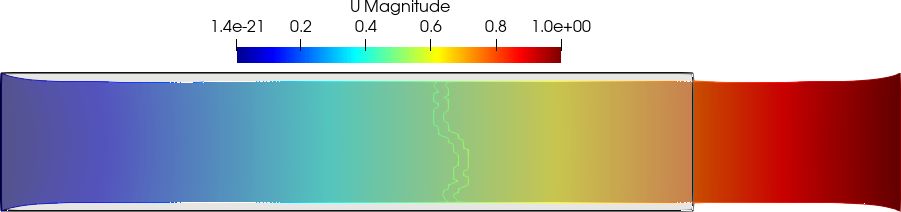
\includegraphics[align=t,width=1\textwidth]{2d-bar-clamped-pulled.png}
    \end{minipage}
    \caption{2D bar results. Partitioned mesh (left) and 1.5X warped displacement field (right).}
    \label{fig:2part}
\end{figure}

Note now in~\cref{fig:2part} there are only two subdomais in the partitioned mesh since only three cores were used. As expected we see that the right end of the bar which is being pulled does not contract in $y$ direction.
\pagebreak


\subsection{PSD simulation of 2D bar problem clamped at one end wile being pulled at the other end (Dirichlet-Neumann case)\label{sec:2d-bar-clamped3}}


Similar simulation, as in \cref{sec:2d-bar-clamped2} is presented in this section. We showcase the 2D bar problem simulation with one end clamped wile being pulled at the other end. Just like simulation from \cref{sec:2d-bar-clamped2} the body force is neglected, However now  the non clamped ends pull is approximated with Neumann force $\int_{\partial\Omega^h_{\text N}}(\mathbf t\cdot \bvh)$. To simulate the pull we assume traction vector $\mathbf t=[t_1,t_2]=[10^9.,0]$ acting on the non clamped right end of the bar, i.e., force in $x$ direction is 10 units. Here is how PSD simulation of this case can be performed.

\textbf{Step 1: Preprocessing}

For ``PSD setup" go to the {\ttfamily PSD/Solver} folder, launch the terminal there and run the following command.
\begin{lstlisting}[style=Linux]
PSD_PreProcess -dimension 2 -dirichletconditions 1  -tractionconditions 1 -plot
\end{lstlisting}
%
the comandline flag {\ttfamily -dirichletconditions 1}, notifies to PSD that there is one Dirichlet border ---the clamped end of the bar--- in this simulation. And the flag {\ttfamily -tractionconditions 1} notifies to PSD that there is one traction border ---the right end of the bar--- in this simulation. 
To add the values and label numbers of the Dirichlet borders edit the  {\ttfamily ControlParameters.edp},  the vector {\ttfamily int[int] Dlabel = [2];} should be used, here we assume that the label number of the left end is 2. For the left end $u_1=0,u_2=0$ hence in {\ttfamily ControlParameters.edp}, use {\ttfamily real[int]   Dvalue = [0.,0.];}. To add the values and label numbers of the traction borders edit the  {\ttfamily ControlParameters.edp},  the vector {\ttfamily int[int] Tlabel = [4];} should be used, here we assume that the label number of the right end is 4. For this end $\mathbf t=[t_1,t_2]=[10^9.,0]$, hence in {\ttfamily ControlParameters.edp}, use {\ttfamily real  tx0=1.e9, ty0=0.;}. 


\textbf{Step 2: Solving}

Let us now use 5 cores to solve this problem. To do so enter the following command:

\begin{lstlisting}[style=Linux]
ff-mpirun -np 5 Main.edp
\end{lstlisting}
%
Notice, that this is the exact same command used in solving the previous bar problems from other sections, with only difference that we now use {\ttfamily -np 5}.


\textbf{Step 3: Postprocessing}

Launch ParaView and have a look at the  {\ttfamily .pvd} file in the  {\ttfamily PSD/Solver/VTUs\_DATE\_TIME} folder. 

\begin{figure}[htbp]
    \centering
    \begin{minipage}[t][2cm][t]{0.36\textwidth}
    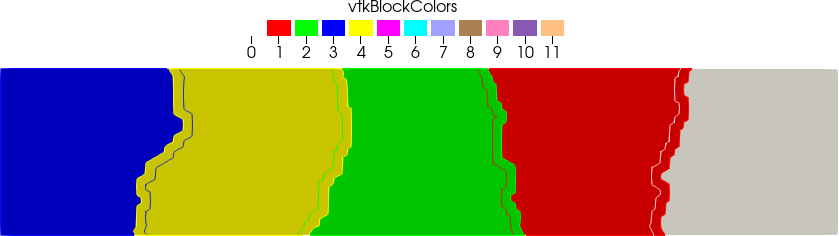
\includegraphics[align=b,width=1\textwidth]{2d-bar-partitioned5.png}
    \end{minipage}\hspace{.1\textwidth}
    \begin{minipage}[t][2cm][t]{0.5\textwidth}
    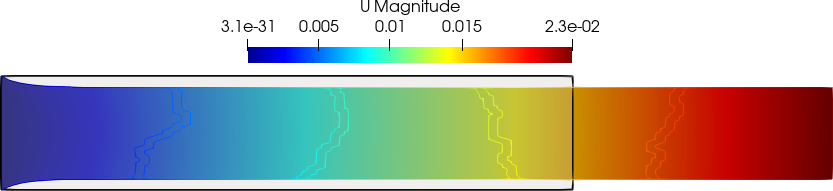
\includegraphics[align=b,width=1\textwidth]{2d-bar-clamped-traction.png}
    \end{minipage}
    \caption{2D bar results. Partitioned mesh (left) and 100X warped displacement field (right).}
    \label{fig:5part}
\end{figure}

Note now in~\cref{fig:5part} there are five subdomais in the partitioned mesh since five cores were used. Contrary to~\cref{fig:2part}, as expected, we see that the right end of the bar which is being pulled now contract in $y$ direction. This is due to the fact that there is no Dirichlet condition at this end now. 

\pagebreak




\subsection{PSD simulation of 2D bar problem clamped at one end wile being pulled at the other end (Dirichlet-Neumann-Point boundary conditions case)\label{sec:2d-bar-clamped4}}


Similar simulations, as in \cref{sec:2d-bar-clamped2,sec:2d-bar-clamped3} is presented in this section. We showcase the 2D bar problem simulation with one end clamped  wile being pulled at the other end. Contrary to simulation in \cref{sec:2d-bar-clamped2,sec:2d-bar-clamped3}, the clamped end just restricts $x$ movement, i.e, $u_1=0$. Just like simulation from \cref{sec:2d-bar-clamped2,sec:2d-bar-clamped3} the body force is neglected. Just like simulation in  \cref{sec:2d-bar-clamped3}, the non clamped ends pull is approximated with Neumann force $\int_{\partial\Omega^h_{\text N}}(\mathbf t\cdot \bvh)$. To simulate the pull we assume traction vector $\mathbf t=[t_1,t_2]=[10^9,0]$ acting on the non clamped right end of the bar, i.e., force in $x$ direction is $10^9$ units. Here is how PSD simulation of this case can be performed.


\textbf{Step 1: Preprocessing}

For ``PSD setup" go to the {\ttfamily PSD/Solver} folder, launch the terminal there and run the following command.
\begin{lstlisting}[style=Linux]
PSD_PreProcess -dimension 2 -dirichletconditions 1 -tractionconditions 1 -dirichletpointconditions 1 -plot
\end{lstlisting}

Additional flag {\ttfamily -dirichletpointconditions 1} now appears, this notifies to PSD that there is one Dirichlet point boundary condition. To add the values and label numbers of the Dirichlet borders which contains this point edit the  {\ttfamily ControlParameters.edp},  the vector {\ttfamily int[int] Dpointlab = [2];} should be used, here we assume that the label number of the left end is 2 and that left end contains our Dirichlet point. For this point $x=y=0$ and $u_1=0,u_2=0$ to specify this in {\ttfamily ControlParameters.edp}, use {\ttfamily PnV = [ 0., 0., 0., 0.];} which is infact a vector of $[x,y,u_1,u_2]$. Via the flags we specified that {\ttfamily -dirichletconditions 1}, i.e., there is one Dirichlet border. However now in this simulation the border only has one Dirichlet condition $u_1=0$, while $u_2$ is free. This condition needs editing of {\ttfamily VariationalFormulations.edp}, comment or remove the line {\ttfamily u1 = Dvalue[1]}. Commenting or removing this line lets free {\ttfamily u1} which is infact $u_2$. Note that this is due to the fact that in PSD $[u_1,u_2,u_3]$ maps to {\ttfamily [u,u1,u2]}.

\textbf{Step 2: Solving}

Let us now use 6 cores to solve this problem. To do so enter the following command:

\begin{lstlisting}[style=Linux]
ff-mpirun -np 5 Main.edp
\end{lstlisting}
%
Notice, that this is the exact same command used in solving the previous bar problems from other sections, with only difference that we now use {\ttfamily -np 6}.


\textbf{Step 3: Postprocessing}

Launch ParaView and have a look at the  {\ttfamily .pvd} file in the  {\ttfamily PSD/Solver/VTUs\_DATE\_TIME} folder. 

\begin{figure}[htbp]
    \centering
    \begin{minipage}[t][2cm][t]{0.36\textwidth}
    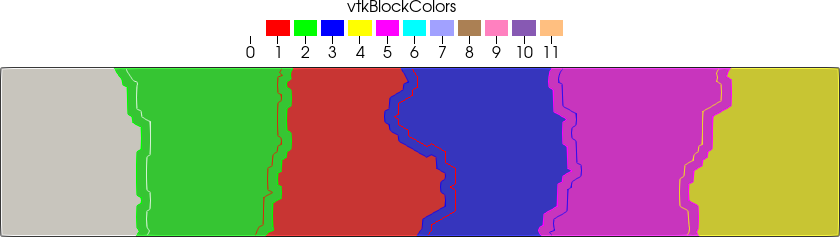
\includegraphics[align=b,width=1\textwidth]{2d-bar-partitioned6.png}
    \end{minipage}\hspace{.1\textwidth}
    \begin{minipage}[t][2cm][t]{0.5\textwidth}
    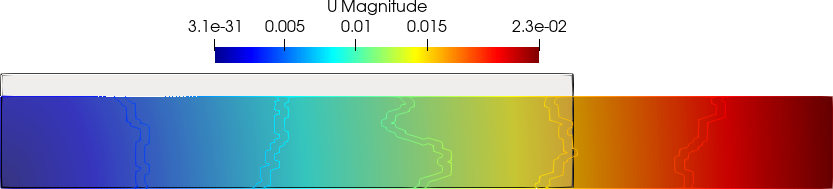
\includegraphics[align=b,width=1\textwidth]{2d-bar-clamped-traction-point.png}
    \end{minipage}
    \caption{2D bar results. Partitioned mesh (left) and 100X warped displacement field (right).}
    \label{fig:6part}
\end{figure}

Note now in~\cref{fig:6part} there are six subdomais in the partitioned mesh. As expected, we see that the right and the left end of the bar which is being pulled now contract in $y$ direction, and the bar elongates in $x$ direction. 






\subsection{PSD simulation of 3D bar problem clamped at one end wile being pulled at the other end (Dirichlet-Neumann case)\label{sec:3d-bar-clamped3}}

In this section we present a 3D PSD simulation of a clamped bar which his being loaded in vertical direction at the non-clamped end. This simulation is like the one presented in \cref{sec:2d-bar-clamped3}, however in 3D. The material properties are same as before, and at the non-clamped end traction $t_y=-10^9$ units. The 3D bar is $1\times1\times5$ m$^3$.

Here is how PSD simulation of this case can be performed.

\textbf{Step 1: Preprocessing}

For ``PSD setup" go to the {\ttfamily PSD/Solver} folder, launch the terminal there and run the following command.
\begin{lstlisting}[style=Linux]
PSD_PreProcess -dimension 3 -dirichletconditions 1  -tractionconditions 1 -plot
\end{lstlisting}
%
the comandline flag {\ttfamily -dirichletconditions 1} notifies to PSD that there is one Dirichlet border ---the clamped end of the bar--- in this simulation; {\ttfamily -dimension 3} means the simulation is 3D. And the flag {\ttfamily -tractionconditions 1} notifies to PSD that there is one traction border ---the right end of the bar--- in this simulation. 
To add the values and label numbers of the Dirichlet borders edit the  {\ttfamily ControlParameters.edp},  the vector {\ttfamily int[int] Dlabel = [1];} should be used, here we know that the label number of the left clamped end is 1. For the left end $u_1=0,u_2=0,u_3=0$ hence in {\ttfamily ControlParameters.edp}, use {\ttfamily real[int]   Dvalue = [0.,0.,0.];}. To add the values and label numbers of the traction borders edit the  {\ttfamily ControlParameters.edp},  the vector {\ttfamily int[int] Tlabel = [2];} should be used, here we know that the label number of the right end is 2. For this end $\mathbf t=[t_1,t_2,t_3]=[0.,10^9,0.]$, hence in {\ttfamily ControlParameters.edp}, use {\ttfamily real  tx0=0., ty0=1.e9, tz0=0.,;}. 


\textbf{Step 2: Solving}

Let us now use 4 cores to solve this problem. To do so enter the following command:

\begin{lstlisting}[style=Linux]
ff-mpirun -np 4 Main.edp
\end{lstlisting}
%
Notice, that this is the exact same command used in solving the previous bar problems from other sections.


\textbf{Step 3: Postprocessing}

Launch ParaView and have a look at the  {\ttfamily .pvd} file in the  {\ttfamily PSD/Solver/VTUs\_DATE\_TIME} folder. 

\begin{figure}[htbp]
    \centering
    \begin{minipage}[t][2cm][t]{0.38\textwidth}
    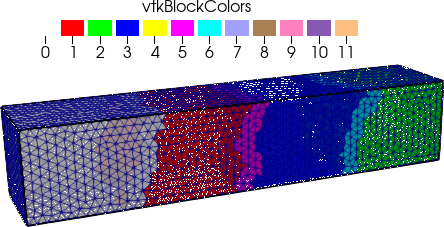
\includegraphics[align=b,width=1\textwidth]{3d-bar-clamped-ends.png}
    \end{minipage}\hspace{.1\textwidth}
    \begin{minipage}[t][2cm][t]{0.4\textwidth}
    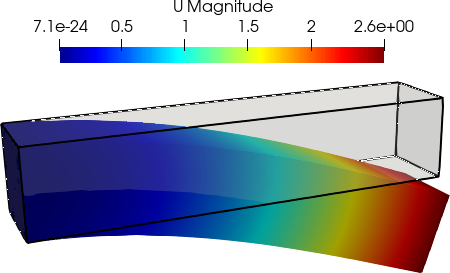
\includegraphics[align=b,width=1\textwidth]{3d-bar-clamped-pulled-partioned.png}
    \end{minipage}
    \caption{3D bar results. Partitioned mesh (left) and 0.5X warped displacement field (right).}
    \label{fig:3Dpart}
\end{figure}

In~\cref{fig:3Dpart} there are four subdomais in the partitioned mesh since four cores were used.

\pagebreak


\subsection{PSD simulation of 3D  mechanical piece (Dirichlet-Neumann case) with complex mesh\label{sec:3d-bar-clamped3}}

So far in the previous cases we only concentrated on bar simulations, which were more or less trivial cases. Moreover, the bar meshes are provided with the PSD solver. In this section we now turn towards  3D simulation of a mechanical piece, the geometry of which is shown in~\cref{fig:mechanicalpiecegeo}. The left (small) hole is fixed: $u_1=u_2=u_3=0$, while as traction force $t_x=10^9$ is applied on the large hole.

You can grab a copy of CAD geometry for the mechanical piece (the Gmsh {\ttfamily .geo}) your local Gmsh installation folder  {\ttfamily gmsh/share/doc/gmsh/demos/simple\_geo/{piece}.geo}. The listing of the file is also given in @. To generate the mesh {\ttfamily piece.msh} simply do 
\begin{lstlisting}[style=Linux]
gmsh -3 piece.geo
\end{lstlisting}
Place the generated mesh {\ttfamily piece.msh} in {\ttfamily /PSD/Meshes/3D/piece.msh}. Now the PSD simulation can be performed.

\begin{figure}[h]
    \centering
    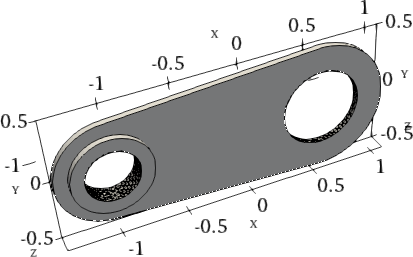
\includegraphics[align=b,width=0.5\textwidth]{3d-mechanical.png}
    \caption{3D mechanical piece.}
    \label{fig:mechanicalpiecegeo}
\end{figure}

\textbf{Step 1: Preprocessing}

For ``PSD setup" go to the {\ttfamily PSD/Solver} folder, launch the terminal there and run the following command.
\begin{lstlisting}[style=Linux]
PSD_PreProcess -dimension 3 -dirichletconditions 1  -tractionconditions 1 -plot
\end{lstlisting}
Here, by using these parameters we have generated one Dirichelet condition and one traction condition, respectively to be applied to the small and the large holes in the mesh. Further, by using {\ttfamily -dimension 3} we have let PSD know that the problem is 3D .In the {\ttfamily /PSD/Meshes/3D/piece.msh} generated, the label 4 (resp.~3) corresponds to the Dirichlet (resp.~traction) border. To add the values and label numbers of the Dirichlet borders edit the  {\ttfamily ControlParameters.edp},  the vector {\ttfamily int[int] Dlabel = [4];} should be used. For this label $u_1=0,u_2=0,u_3=0$ hence in {\ttfamily ControlParameters.edp}, use {\ttfamily real[int]   Dvalue = [0.,0.,0.];}. To add the values and label numbers of the traction borders edit the  {\ttfamily ControlParameters.edp},  the vector {\ttfamily int[int] Tlabel = [3];} should be used. For this end $\mathbf t=[t_1,t_2,t_3]=[0.,10^9,0.]$, hence in {\ttfamily ControlParameters.edp}, use {\ttfamily real  tx0=0., ty0=1.e9, tz0=0.,;}. Finally we use steel properties for the material, so in {\ttfamily ControlParameters.edp} the parameters {\ttfamily real E  = 200.e9;} and {\ttfamily real nu = 0.3;} should be used. These represent $E$ and $\nu$, respectively. With all the properties and boundary conditions set we now use  {\ttfamily string ThName = "../Meshes/3D/piece";} in the {\ttfamily ControlParameters.edp} file, this notifies PSD about the name of the mesh used for this simulation.  

\textbf{Step 2: Solving}

Let us now use 2 cores to solve this problem. To do so enter the following command:

\begin{lstlisting}[style=Linux]
ff-mpirun -np 2 Main.edp
\end{lstlisting}

\textbf{Step 3: Postprocessing}

Launch ParaView and have a look at the  {\ttfamily .pvd} file in the  {\ttfamily PSD/Solver/VTUs\_DATE\_TIME} folder. 

\begin{figure}[htbp]
    \centering
    \begin{minipage}[t][2cm][t]{0.36\textwidth}
    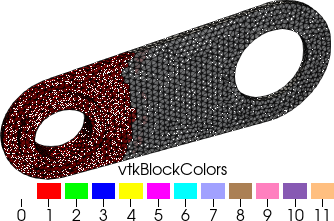
\includegraphics[align=b,width=1\textwidth]{3d-mechanical-part.png}
    \end{minipage}\hspace{.1\textwidth}
    \begin{minipage}[t][2cm][t]{0.4\textwidth}
    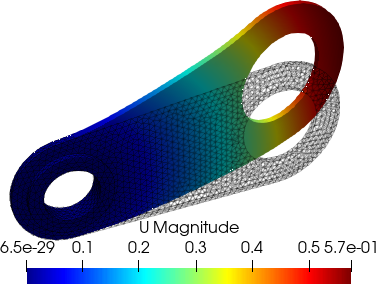
\includegraphics[align=b,width=1\textwidth]{3d-mechanical-result.png}
    \end{minipage}
    \caption{Mechanical piece test results. Partitioned mesh (left) and  warped displacement field (right).}
    \label{fig:mechapieceresult}
\end{figure}

\textbf{Redoing the test with different conditions}

\begin{figure}[htbp]
    \centering
    \begin{minipage}{0.42\textwidth}
    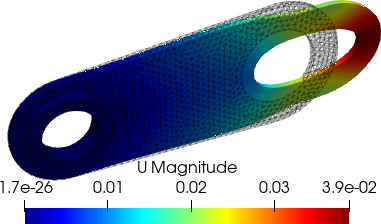
\includegraphics[align=b,width=1\textwidth]{3d-mechanical-result-x.png}
    \subcaption{{\ttfamily real  tx0=1.e9, ty0=0, tz0=0.,;}}
    \end{minipage}\hspace{.1\textwidth}
    \begin{minipage}{0.4\textwidth}
    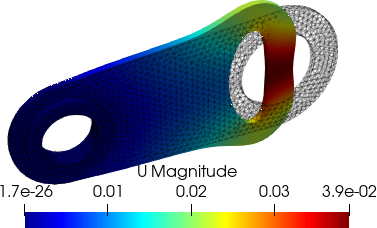
\includegraphics[align=b,width=1\textwidth]{3d-mechanical-result--x.png}
    \subcaption{{\ttfamily real  tx0=1.e9, ty0=0, tz0=0.,;}}
    \end{minipage}
    \caption{Mechanical piece test results.}
    \label{fig:mechapieceresult2}
\end{figure}



\pagebreak













\section{Damage mechanics}
\subsection{Hybrid phase-field for damage}
On a meshed domain $\Omega^h\in\Omega\subset\mathbb{R}^n$, for damage mechanics the mixed finite element variational formulation in the Lagrangian framework for searching the unknown nodal displacements vector $\bu^h=[u_1,u_2,u_3]^\mathsf{T}$ reads,
%
%
\begin{equation}\label{Eq:VarfU}
\begin{aligned}
&\text{search}~\buh\in\mathbb{V}^h \text{~that satisfies}~\forall\, t\in[0,T]:\\
&\int_{\Omega^h}\big[(1-d^h)^2 + \kappa \big]\sig(\buh) : \eps(\bvh) \,\dv= \int_{\partial\Omega^h_\text{N}} \overline{\bt}\cdot\bvh \,\ds \quad\forall\,\bv^h\in\mathbb{V}^h,
\end{aligned}
\end{equation}
where $\kappa\ll1$ is a model parameter to prevent numerical singularity when $d \to 1$.
 %
 %
In this formulation, the notation ``$:$" is used for the double contraction between tensors (i.e., component-wise tensor product) and $ \mathbb{V}^h $ is a  mixed third order vector valued finite element functional space to approximate vector test function~$\bvh$ and vector trial function~$\buh$:
 %
\begin{equation}
\mathbb{V}^h=\left\{ \bu^h\in [ {H}^1(\Omega^h) ]^3~~\forall t\in[0,T]~|~ \forall \bx\in\partial\Omega^h_{\text{D}}~\buh=\overline{\bu}\right\},
\end{equation}
%
with ${H}^1(\Omega^h)$ denoting a square integrable Sobolev functional space.
Similarly, for~the phase-field the standard finite element variational formulation for the unknown damage scalar $\fih$ reads, 
%
%
\begin{equation}
\begin{aligned}\label{Eq:VarfPhi}
&\text{search}~\fih\in{{V}}^h \text{~that satisfies}~\forall\, t\in[0,T]:\\
&\int_{\Omega^h}\left[ \frac{\bgc}{l_0} + 2 \mathcal{H}^{+}(\buh) \right]\fih\ttah\, \dv + \int_{\Omega^h} {\bgc}{l_0}\nabla\fih \cdot \nabla\ttah \, \dv= \int_{\Omega^h} 2\mathcal{H}^{+}(\buh)\ttah \, \dv\quad\forall\,\ttah\in{{V}}^h, 
\end{aligned}
\end{equation}
%
%
where,~${{V}}^h$ denotes the scalar finite element functional space to approximate scalar test function~$\ttah$ and scalar trial function~$\fih$:
\begin{equation}
{{V}}^h=\left\{\fih \in  {H}^1(\Omega^h)~~\forall t\in[0,T]~\middle|~\fih\in[0,1]  \right\}.
\end{equation}


\lstset{
  language={PSD},
  basicstyle=\small\ttfamily, % Global Code Style
  captionpos=b, % Position of the Caption (t for top, b for bottom)
  extendedchars=true, % Allows 256 instead of 128 ASCII characters
  tabsize=2, % number of spaces indented when discovering a tab 
  columns=fixed, % make all characters equal width
  keepspaces=true, % does not ignore spaces to fit width, convert tabs to spaces
  showstringspaces=false, % lets spaces in strings appear as real spaces
  breaklines=true, % wrap lines if they don't fit
  frame=trbl, % draw a frame at the top, right, left and bottom of the listing
  frameround=tttt, % make the frame round at all four corners
  framesep=4pt, % quarter circle size of the round corners
  numbers=left, % show line numbers at the left
  numberstyle=\tiny\ttfamily, % style of the line numbers
  commentstyle=\color{eclipseGreen}, % style of comments
  keywordstyle=\color{eclipsePurple}, % style of keywords
  stringstyle=\color{eclipseBlue}, % style of strings
}



\begin{lstlisting}[language=PSD]
import math
import numpy as np
from lib.analytical import csa

sin2_theta  = np.sin(theta)**2  // THis is  a commen
+= -= *= /= + - * / ? < > & % == <=
# += -= *= /= + - * / ? < > & % == <=
def test(a=100, b=True):
    <= >= == 2 + 3j * 7e-3
\end{lstlisting}

\chapter{Validation}


\chapter{Functions and descriptions}

\chapter{Gallery}

This chapter showcases some test cases that have been peformed with PSD.


\end{document}